%& -shell-escape -enable-write18 
\documentclass[uplatex,dvipdfmx]{jsarticle}
\usepackage[utf8]{inputenc}

\usepackage[dvipdfmx]{graphicx}
\usepackage[dvipdfmx]{color}
\usepackage[driver=dvipdfm,hmargin=19.05truemm,vmargin=25.40truemm]{geometry}
\usepackage{colortbl}
\usepackage{tcolorbox}
\usepackage{varwidth}
\usepackage{xcolor}
\PassOptionsToPackage{dvipsnames}{xcolor}

\usepackage{amsmath,amsfonts,amssymb,amsthm}
\usepackage{bm}
\usepackage[italicdiff]{physics}
\usepackage{mathtools}
\mathtoolsset{showonlyrefs=true}
\usepackage[unicode, dvipdfmx]{hyperref}
\usepackage{pxjahyper}
\hypersetup{
setpagesize=false,
    bookmarksnumbered=true,
    bookmarksopen=true,
    colorlinks=true,
    linkcolor=cyan,
    citecolor=red,
}
\usepackage{mathrsfs}
\usepackage{bussproofs}
\usepackage{enumerate}
\usepackage{pxrubrica}
\usepackage{tipa}
\usepackage{ascmac}
\usepackage{caption}
\usepackage[subrefformat=parens]{subcaption}
\usepackage{listings,jvlisting}
\usepackage{tikz}
\usetikzlibrary{math,patterns,intersections,calc,arrows,graphs}
\usepackage{float}
\usepackage{xparse}
\usepackage{url}
\usepackage{fancyhdr}
\usepackage{multicol}
\usepackage{siunitx}
\usepackage{hhline}
\usepackage{bxbase}
\usepackage[mark=***]{sectionbreak}
\usepackage[geometry]{ifsym}
\usepackage[prefernoncjk]{pxcjkcat}
\usepackage[LGR,T2A,T3,T1]{fontenc}
\usepackage[greek,latin,english,russian,japanese]{pxbabel}

\allowdisplaybreaks


\theoremstyle{definition}
\newtheorem{theorem}{Thm}
\newtheorem{corollary}{Col}
\newtheorem{lemma}{Lem}
\newtheorem{definition}{Def}
\newtheorem{proposition}{Prop}

\tcbuselibrary{most}

\renewcommand{\labelitemi}{$\circ$}
\renewcommand{\labelitemii}{$\triangleright$}

\ProvideDocumentCommand\floor{m}{\lfloor {#1} \rfloor}
\ProvideDocumentCommand{\where}{}{\mathrel{}\middle|\mathrel{}}
\ProvideDocumentCommand{\when}{m}{\quad({#1})}
\ProvideDocumentCommand{\adjoint}{}{\mathbf{\ast}}
\ProvideDocumentCommand{\conjugation}{}{\mathbf{\ast}}
\NewDocumentCommand{\Jacobi}{m m}{\frac{\partial ({#1})}{\partial ({#2})}}
\NewDocumentCommand{\JacobiPolar}{O{x,y}}{\frac{\partial ({#1})}{\partial (r,\theta)}}
\DeclareMathOperator{\Ker}{Ker}
\DeclareMathOperator{\Img}{Im}
\DeclareMathOperator{\res}{Res}
\DeclareMathOperator{\Dom}{Dom}
\DeclareMathOperator{\Ran}{Ran}

\DeclareMathOperator{\exd}{d}

\DeclareFontShape{JY2}{mc}{m}{it}{<->ssub*mc/m/n}{}
\DeclareFontShape{JY2}{mc}{m}{sl}{<->ssub*mc/m/n}{}
\DeclareFontShape{JY2}{mc}{m}{sc}{<->ssub*mc/m/n}{}
\DeclareFontShape{JY2}{gt}{m}{it}{<->ssub*gt/m/n}{}
\DeclareFontShape{JY2}{gt}{m}{sl}{<->ssub*gt/m/n}{}
\DeclareFontShape{JY2}{mc}{b}{it}{<->ssub*mc/bx/it}{}
\DeclareFontShape{JY2}{mc}{bx}{it}{<->ssub*gt/m/n}{}
\DeclareFontShape{JY2}{mc}{bx}{sl}{<->ssub*gt/m/n}{}
\DeclareFontShape{JT2}{mc}{m}{it}{<->ssub*mc/m/n}{}
\DeclareFontShape{JT2}{mc}{m}{sl}{<->ssub*mc/m/n}{}
\DeclareFontShape{JT2}{mc}{m}{sc}{<->ssub*mc/m/n}{}
\DeclareFontShape{JT2}{gt}{m}{it}{<->ssub*gt/m/n}{}
\DeclareFontShape{JT2}{gt}{m}{sl}{<->ssub*gt/m/n}{}
\DeclareFontShape{JT2}{mc}{b}{it}{<->ssub*gt/b/n}{}
\DeclareFontShape{JT2}{mc}{bx}{it}{<->ssub*gt/m/n}{}
\DeclareFontShape{JT2}{mc}{bx}{sl}{<->ssub*gt/m/n}{}

\DeclareFontShape{J30}{mc}{b}{it}{<->ssub*mc/bx/it}{}
\DeclareFontShape{J30}{mc}{b}{n}{<->ssub*mc/bx/n}{}
\DeclareFontShape{J20}{mc}{b}{it}{<->ssub*mc/bx/it}{}
\DeclareFontShape{J20}{mc}{b}{n}{<->ssub*mc/bx/n}{}
\ProvideDocumentCommand{\titleof}{m}{

\title{ここに講義タイトルを入力 \\ {#1}レポート課題}
\author{ここに名前を入力}
\date{}
}
\titleof{10/12}

\begin{document}

\maketitle

\begin{enumerate}[(1)]
    \item 
    \begin{enumerate}[(i)]
        \item $c\ge 0$をとる.$\displaystyle \lim_{n\to\infty}f_n(c)=\lim_{n\to\infty}\dfrac{1}{1+c^n}$は存在して,
        \begin{equation}
            \lim_{n\to\infty}f_n(c)
            =
            \begin{dcases}
                1          &((0\le)c<1)\\
                \frac{1}{2}&(c=1)\\
                0          &(c>1)
            \end{dcases}
        \end{equation}
        となるから関数列$\qty{f_n}$は各点収束で,
        \begin{equation}
            f(x)
            =
            \begin{dcases}
                1          &((0\le)x<1)\\
                \frac{1}{2}&(x=1)\\
                0          &(x>1)
            \end{dcases}
        \end{equation}
        である.図示すると以下のようになる.
        \begin{figure}[H]
            \centering
            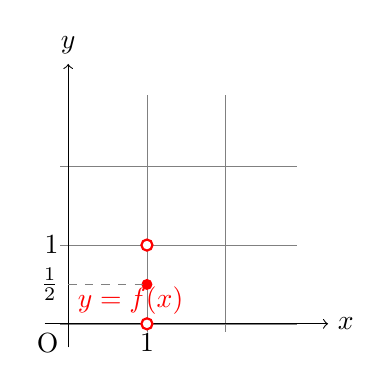
\begin{tikzpicture}[domain=0:3]

                \draw[very thin,color=gray] (-0.1,-0.1) grid (2.9,2.9);
                \draw[->] (-0.3,0) -- (3.3,0) node[right] {$x$};
                \draw[->] (0,-0.3) -- (0,3.3) node[above] {$y$};
                
                \draw (0,0) node[below left] {$\mathrm{O}$};
                \draw (1,0) node[below] {$1$};
                \draw (0,1) node[left] {$1$};
                \draw (0,0.5) node[left] {$\frac{1}{2}$};

                \draw[domain=0:1,color=red] plot[id=1] function{1} ;
                \filldraw[draw=red, thick,fill=white] (1,1) circle (2pt);
                \fill[red] (1,0.5) circle [radius=2pt];
                \draw[dashed,very thin,color=gray] (0,0.5) -- (1,0.5);
                \filldraw[draw=red, thick,fill=white] (1,0) circle (2pt);
                \draw[domain=1:3,color=red] plot[id=1] function{0} node[above right] {$y=f(x)$};

            \end{tikzpicture}
        \end{figure}
        \item 関数列$\qty{f_n}$が$I\in\qty[a,b]$で絶対収束する点$\qty(a,b)$の範囲は,
        \begin{gather}
            1<a<b,(0\le)a<b<1
        \end{gather}
        である.これを図示すると以下のようになる.ただし,境界は$b$軸との共通部分のみ含む.
        \begin{figure}[H]
            \centering
            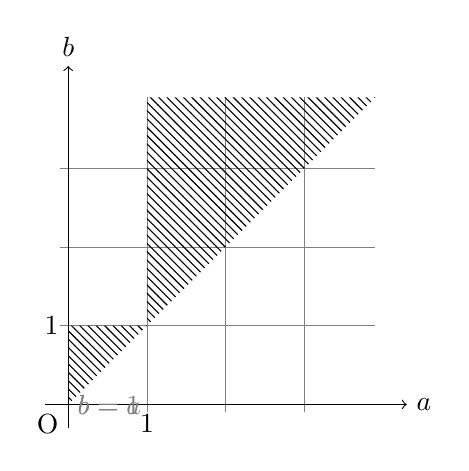
\begin{tikzpicture}[domain=0:4]
                
                \draw[very thin,color=gray] (-0.1,-0.1) grid (3.9,3.9);
                \draw[->] (-0.3,0) -- (4.3,0) node[right] {$a$};
                \draw[->] (0,-0.3) -- (0,4.3) node[above] {$b$};
                
                \draw (0,0) node[below left] {$\mathrm{O}$};
                \draw (1,0) node[below] {$1$};
                \draw (0,1) node[left] {$1$};

                \fill[pattern=north west lines]
                    (0,0)--(1,1)--(0,1);
                \fill[pattern=north west lines]
                    (1,1)--(3.9,3.9)--(1,3.9)--(1,1);
                
                \draw[domain=0:4,dashed,very thin,color=gray] plot[id=x] function{x} node[right] {$b=a$};
                \draw[domain=0:4,dashed,very thin,color=gray] plot[id=1] function{1} node[right] {$b=1$};

            \end{tikzpicture}
        \end{figure}
        \begin{itemize}
            \item $a>1$のとき\\
            \begin{align}
                \sup_{x\in I}\abs{f_n(x)-f(x)}
                &=\sup_{x\in I}\frac{1}{1+x^n}\\
                &=\frac{1}{1+a^n}\\
                &\to 0& (n\to\infty)
            \end{align}
            となるから,一様収束する.
            \item $a=1$のとき\\
            \begin{align}
                \sup_{x\in I}\abs{f_n(x)-f(x)}
                &=\sup_{x\in I}\frac{1}{1+x^n}\\
                &=\frac{1}{1+1^n}\\
                &=\frac{1}{1+1}\\
                &=\frac{1}{2}
            \end{align}
            であるから,たとえば$\varepsilon = \dfrac{1}{4}$とすれば任意の$N\in\mathbb{N}$に対して$n>N$のとき
            \begin{equation}
                \sup_{x\in I}\abs{f_n(x)-f(x)}\ge \varepsilon
            \end{equation}
            が成り立つため一様収束しない.
            \item $(0\le)a<1$のとき
            \begin{itemize}
                \item $b\ge 1$のとき
                \begin{align}
                    \sup_{x\in I}\abs{f_n(x)-f(x)}
                    &=\sup_{x\in I}\dfrac{1}{1+x^n}\\
                    &=\dfrac{1}{1+1^n}\\
                    &=\dfrac{1}{1+1}\\
                    &=\dfrac{1}{2}
                \end{align}
                である.$a=1$のときと同一の議論で一様収束しないことが示される.
                \item $b<1$のとき
                \begin{align}
                    \sup_{x\in I}\abs{f_n(x)-f(x)}
                    &=\sup_{x\in I}\dfrac{x^n}{1+x^n}\\
                    &=\dfrac{b^n}{1+b^n}\\
                    &\to 0& (n\to\infty)
                \end{align}
                となるから,一様収束する.
            \end{itemize}
        \end{itemize}
    \end{enumerate}
    \begin{enumerate}[(i)]
        \item 両辺を$t^3+1$で乗じると両辺とも多項式になるため,$t$の次数ごとに係数比較すると,
        \begin{align}
            &\begin{dcases}
                A+2B&=0\\
                -A+B+C&=0\\
                A-B+C&=1
            \end{dcases}
            \\
            &\begin{dcases}
                A&=\frac{1}{3}\\
                A&=-\frac{1}{6}\\
                A&=\frac{1}{2}
            \end{dcases}
        \end{align}
        であるから,
        \begin{align}
            \int_0^x\frac{1}{t^3+1}dt
            &=\frac{1}{3}\int_0^x \frac{1}{t+1} dt
            -\frac{1}{6}\int_0^x \frac{(t^2-t+1)^\prime}{t^2-t+1} dt
            +\frac{1}{2}\int_0^x \frac{1}{t^2-t+1} dt\\
            &=\frac{1}{3}\log(x+1)
            -\frac{1}{6}\log(x^2-x+1)
            +\frac{1}{2}\int_0^x \frac{1}{(t-\frac{1}{2})^2+\frac{3}{4}} dt
        \end{align}
        である.ここで
        \begin{align}
            \dv{t}(\arctan\frac{t}{a})&=\frac{a}{t^2+a^2}\\
            \therefore \dv{t}(\arctan\frac{t-\frac{1}{2}}{a})&=\frac{a}{(t-\frac{1}{2})^2+a^2}
        \end{align}
        により
        \begin{align}
            \int_0^x\frac{1}{t^3+1}dt
            &=\frac{1}{3}\log(x+1)
            -\frac{1}{6}\log(x^2-x+1)
            +\frac{1}{2}\int_0^x \frac{1}{(t-\frac{1}{2})^2+\frac{3}{4}} dt\\
            &=\frac{1}{3}\log(x+1)
            -\frac{1}{6}\log(x^2-x+1)
            +\frac{1}{\sqrt{3}}\arctan\frac{t-\frac{1}{2}}{\frac{\sqrt{3}}{2}}\evaluated{}_{t=0}^x\\
            &=\frac{1}{3}\log(x+1)
            -\frac{1}{6}\log(x^2-x+1)
            +\frac{1}{\sqrt{3}}\qty(\arctan\frac{x-\frac{1}{2}}{\frac{\sqrt{3}}{2}}+\frac{\pi}{6})\label{eq:fx}
        \end{align}
        である.
        \item $\displaystyle\sum_{n=0}^{\infty}\frac{1}{3n+1}$は発散し,$\displaystyle\sum_{n=0}^{\infty}\frac{(-1)^n}{3n+1}=\frac{1}{3}\log2
        +\frac{\pi}{3\sqrt{3}}$である.
        \begin{itemize}
            \item $\displaystyle\sum_{n=0}^{\infty}\frac{1}{3n+1}$について\\
            $\dfrac{1}{3n+1}>\dfrac{1}{3(n+1)}$であり,
            \begin{equation}
                \sum_{n=0}^{m}\frac{1}{3(n+1)}
                =\frac{1}{3}\sum_{n=1}^{m}\frac{1}{n}
            \end{equation}
            右辺は$n\to\infty$の極限で発散するので,
            \begin{equation}
                \displaystyle\sum_{n=0}^{\infty}\frac{1}{3n+1}=\infty \qq{(発散)}
            \end{equation}
            である.
            \item $\displaystyle\sum_{n=0}^{\infty}\frac{(-1)^n}{3n+1}$について\\
            $\displaystyle\sum_{n=0}^{\infty}\frac{(-1)^n}{3n+1}$は収束する.なぜなら,$\qty{a_n};a_n=\dfrac{1}{3n+1}$は単調減少数列であり,そして$\displaystyle\lim_{n\to\infty}a_n=0$であり交代級数の収束によりこの級数の収束が従うからである.

            さて,級数$\displaystyle\sum_{n=0}^{\infty}(-1)^n t^{3n}$の収束半径は$1$であるから,これを$t\in\qty[0,x]$で積分した級数$\displaystyle\sum_{n=0}^{\infty}(-1)^n t^{3n}$の収束半径も$1$である.$x<1$のとき
            \begin{align}
                \int_0^x \frac{1}{t^3+1}dt
                &=\sum_{n=0}^\infty\qty(\int_0^x(-1)^nt^{3n}dt)\\
                &=\sum_{n=0}^\infty(-1)^n\frac{1}{3n+1}x^{3n+1}
            \end{align}
            左辺の$x\to 1-0$の極限は\eqref{eq:fx}式に$x:=1$を代入したものであり,これは収束するから,Abelの定理より
            \begin{equation}
                \sum_{n=0}^\infty\frac{(-1)^n}{3n+1}
                =\frac{1}{3}\log2
                +\frac{\pi}{3\sqrt{3}}
            \end{equation}
            である.
        \end{itemize}
    \end{enumerate}
\end{enumerate}

\end{document}